\documentclass[conference]{IEEEtran}

\usepackage{cite}
\usepackage{amsmath,amssymb}
\usepackage{graphicx}
\usepackage{booktabs}
\usepackage{url}
\usepackage{algorithm}
\usepackage{algorithmic}
\usepackage{tikz}
\usetikzlibrary{arrows.meta,positioning}

\newcommand{\E}{\mathbb{E}}
\newcommand{\pdata}{p_{\mathrm{data}}}
\newcommand{\KL}{\mathrm{KL}}
\newcommand{\JSD}{\mathrm{JSD}}

\begin{document}

\title{Generative Adversarial Networks: Mathematical Foundations, Training Dynamics, and Architectural Advances}

\author{\IEEEauthorblockN{Nagham Taweel}
\IEEEauthorblockA{NLP \& AI Internship, Cellula Technologies\\
naghamatawel@gmail.com}}

\maketitle

\begin{abstract}
Generative adversarial networks (GANs) learn to generate realistic data by training two neural networks against each other: a generator that produces samples and a discriminator that tries to tell them apart from real data. This report studies GANs through four papers: the original GAN of Goodfellow et al.\ (2014), the deep convolutional GAN (DCGAN), the Wasserstein GAN (WGAN), and the style-based generator (StyleGAN). Conditional GANs and the gradient-penalty WGAN (WGAN-GP) are treated as extensions. We derive the GAN objective from first principles: the optimal discriminator, the reduction of the generator's objective to the Jensen--Shannon divergence, the global optimum, and its interpretation as a Nash equilibrium. We also derive the gradients behind the vanishing-gradient problem and the non-saturating loss. We then explain the training algorithm and its failure modes (non-convergence, mode collapse, vanishing gradients, and instability), and show mathematically how the Wasserstein distance and the gradient penalty address them. We compare the architectures and their reported results, and review applications in image generation, super-resolution, image-to-image translation, data augmentation, and medical imaging.
\end{abstract}

\begin{IEEEkeywords}
generative adversarial networks, minimax game, Jensen--Shannon divergence, Wasserstein distance, DCGAN, StyleGAN
\end{IEEEkeywords}

\section{Introduction}
A generative model learns the probability distribution of a dataset so that it can produce new samples that look like the data. Before 2014, deep generative models such as deep belief networks relied on approximate likelihoods and Markov chains, which were slow and difficult to train~\cite{goodfellow2014}. Goodfellow et al.\ proposed a different idea: instead of writing down the likelihood, train a generator by letting it compete with a classifier~\cite{goodfellow2014}. The paper explains the idea with an analogy. The generator is like a team of counterfeiters trying to produce fake money, and the discriminator is like the police trying to detect it. Competition drives both to improve until the fakes cannot be distinguished from the real currency.

The idea quickly led to many improvements. Mirza and Osindero added conditioning information, so that a GAN could be told what to generate~\cite{mirza2014}. Radford et al.\ found convolutional architectures that trained stably on images (DCGAN)~\cite{radford2016}. Arjovsky et al.\ replaced the Jensen--Shannon divergence with the Wasserstein distance (WGAN)~\cite{arjovsky2017}, and Gulrajani et al.\ replaced its weight clipping with a gradient penalty (WGAN-GP)~\cite{gulrajani2017}. Karras et al.\ redesigned the generator around style control (StyleGAN), producing photorealistic faces at $1024\times1024$ resolution~\cite{karras2019}.

\textbf{Paper selection.} We analyze four papers in depth. The original GAN~\cite{goodfellow2014} provides the mathematical foundation. DCGAN~\cite{radford2016} is the main architectural improvement for images. WGAN~\cite{arjovsky2017} is the main mathematical improvement for stable training. StyleGAN~\cite{karras2019} represents the modern state of the art in quality and control. Section~II introduces the concepts, Section~III derives the mathematics, Section~IV explains training and its problems, Section~V covers the advanced architectures, and Section~VI reviews applications.

\section{Fundamental Concepts}
A GAN consists of two networks (Fig.~\ref{fig:gan}).

\textbf{Generator $G$.} The generator $G(\mathbf{z};\theta_g)$ maps a random noise vector $\mathbf{z}$, drawn from a simple prior $p_z$ such as a uniform or standard Gaussian distribution, to a sample $\tilde{\mathbf{x}}=G(\mathbf{z})$ in data space, for example an image. The noise vector is called the latent vector, because it acts as a hidden code from which the sample is built. Sampling many vectors $\mathbf{z}$ and passing them through $G$ defines the generator's distribution $p_g$. The goal is to make $p_g$ equal to the real data distribution $\pdata$.

\textbf{Discriminator $D$.} The discriminator $D(\mathbf{x};\theta_d)$ outputs a single number in $[0,1]$: the probability that $\mathbf{x}$ came from the real data rather than from $G$. It is a binary classifier trained on real samples (label 1) and generated samples (label 0).

\textbf{Competition.} The two networks have opposite goals. $D$ is trained to classify correctly, while $G$ is trained to make $D$ classify its samples as real. $G$ never sees real data directly. It learns only through the gradients that flow back through $D$, which tell it how to change its outputs to look more real. When training succeeds, $G$ produces samples that $D$ cannot separate from real data, and $D$ outputs $1/2$ everywhere.

\begin{figure}[t]
\centering
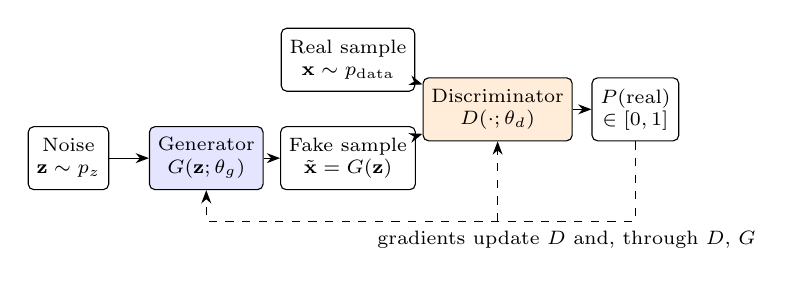
\begin{tikzpicture}[font=\scriptsize, >=Stealth,
  b/.style={draw, rounded corners=2pt, align=center, minimum height=0.8cm, inner sep=3pt}]
\node[b] (z) at (0,0) {Noise\\$\mathbf{z}\sim p_z$};
\node[b, fill=blue!10] (g) at (1.75,0) {Generator\\$G(\mathbf{z};\theta_g)$};
\node[b] (fake) at (3.55,0) {Fake sample\\$\tilde{\mathbf{x}}=G(\mathbf{z})$};
\node[b] (real) at (3.55,1.25) {Real sample\\$\mathbf{x}\sim\pdata$};
\node[b, fill=orange!15] (d) at (5.45,0.62) {Discriminator\\$D(\cdot;\theta_d)$};
\node[b] (out) at (7.2,0.62) {$P(\text{real})$\\$\in[0,1]$};
\draw[->] (z) -- (g);
\draw[->] (g) -- (fake);
\draw[->] (fake) -- (d);
\draw[->] (real) -- (d);
\draw[->] (d) -- (out);
\draw[->, dashed] (out.south) |- (5.45,-0.8) node[pos=0.75, below] {gradients update $D$ and, through $D$, $G$} -| (g.south);
\draw[->, dashed] (5.45,-0.8) -- (d.south);
\end{tikzpicture}
\caption{GAN structure. The discriminator classifies real and generated samples. Its gradients train both networks.}
\label{fig:gan}
\end{figure}

\section{Mathematical Foundations}
\subsection{The Minimax Objective}
The two players optimize one shared value function $V(D,G)$~\cite[Eq.~1]{goodfellow2014}:
\begin{align}
\min_G\max_D V(D,G)={}&\E_{\mathbf{x}\sim\pdata}\!\left[\log D(\mathbf{x})\right]\nonumber\\
&+\E_{\mathbf{z}\sim p_z}\!\left[\log\left(1-D(G(\mathbf{z}))\right)\right].
\label{eq:minimax}
\end{align}
The first term is large when $D$ assigns high probability to real data. The second term is large when $D$ assigns low probability to generated samples. $D$ maximizes $V$, which is the same as minimizing the binary cross-entropy loss of a real-versus-fake classifier. $G$ affects only the second term and minimizes it by making $D(G(\mathbf{z}))$ close to 1. This is a two-player zero-sum game: what one player gains, the other loses.

\subsection{The Optimal Discriminator}
\textbf{Step 1: write $V$ as one integral.} Writing the expectations as integrals, and using the fact that sampling $\mathbf{z}$ and computing $\mathbf{x}=G(\mathbf{z})$ is the same as sampling $\mathbf{x}\sim p_g$, gives
\begin{align}
V(D,G)={}&\int_{\mathbf{x}}\pdata(\mathbf{x})\log D(\mathbf{x})\,d\mathbf{x}\nonumber\\
&+\int_{\mathbf{z}}p_z(\mathbf{z})\log\left(1-D(G(\mathbf{z}))\right)d\mathbf{z}\nonumber\\
={}&\int_{\mathbf{x}}\Big[\pdata(\mathbf{x})\log D(\mathbf{x})+p_g(\mathbf{x})\log\left(1-D(\mathbf{x})\right)\Big]d\mathbf{x}.
\end{align}

\textbf{Step 2: maximize point by point.} For a fixed $G$, $D$ can choose its output separately at every point $\mathbf{x}$. Let $a=\pdata(\mathbf{x})$, $b=p_g(\mathbf{x})$, and $y=D(\mathbf{x})$. The integrand is $f(y)=a\log y+b\log(1-y)$. Setting its derivative to zero,
\begin{equation}
f'(y)=\frac{a}{y}-\frac{b}{1-y}=0\;\Rightarrow\;a(1-y)=by\;\Rightarrow\;y=\frac{a}{a+b}.
\end{equation}
Since $f''(y)=-a/y^2-b/(1-y)^2<0$, this is a maximum. The optimal discriminator is therefore~\cite[Prop.~1]{goodfellow2014}
\begin{equation}
D^*_G(\mathbf{x})=\frac{\pdata(\mathbf{x})}{\pdata(\mathbf{x})+p_g(\mathbf{x})}.
\label{eq:dstar}
\end{equation}
This result has a clear meaning: $D^*$ is the probability that a point came from the data rather than the generator, when both are equally likely a priori. Wherever $p_g=\pdata$, $D^*=1/2$.

\subsection{The Generator's Objective and the Jensen--Shannon Divergence}
\textbf{Step 3: substitute $D^*$.} With the optimal discriminator, the generator minimizes the virtual training criterion $C(G)=\max_D V(D,G)$:
\begin{equation}
C(G)=\E_{\pdata}\!\left[\log\frac{\pdata}{\pdata+p_g}\right]+\E_{p_g}\!\left[\log\frac{p_g}{\pdata+p_g}\right].
\end{equation}

\textbf{Step 4: introduce the mixture.} Let $m=(\pdata+p_g)/2$, so $\pdata+p_g=2m$. Then $\log\frac{\pdata}{2m}=\log\frac{\pdata}{m}-\log2$, and similarly for $p_g$. Each expectation therefore splits into a Kullback--Leibler (KL) divergence minus $\log2$:
\begin{align}
C(G)&=\KL\!\left(\pdata\,\|\,m\right)-\log2+\KL\!\left(p_g\,\|\,m\right)-\log2\nonumber\\
&=-\log4+2\cdot\JSD\!\left(\pdata\,\|\,p_g\right),
\label{eq:jsd}
\end{align}
where $\JSD(P\|Q)=\frac12\KL(P\|m)+\frac12\KL(Q\|m)$ is the Jensen--Shannon divergence~\cite[Thm.~1]{goodfellow2014}.

\textbf{Step 5: the global optimum.} The JSD is always non-negative and equals zero only when the two distributions are identical. Therefore $C(G)\ge-\log4$, with equality if and only if $p_g=\pdata$. At this point, $D^*=1/2$ everywhere and $V=\log\frac12+\log\frac12=-\log4$. Training a GAN with an optimal discriminator thus minimizes a proper distance between the generated and real distributions.

\subsection{Nash Equilibrium Interpretation}
A Nash equilibrium is a pair of strategies in which neither player can improve by changing only its own strategy. For the minimax game in (\ref{eq:minimax}), this is a saddle point $(G^*,D^*)$ satisfying
\begin{equation}
V(D,G^*)\le V(D^*,G^*)\le V(D^*,G)\quad\text{for all }D,G.
\end{equation}
The left inequality says that $D$ cannot gain by deviating, and the right says that $G$ cannot. The derivation above shows that $p_g=\pdata$ with $D=1/2$ is such a point. No generator can do better than reproducing the data, and against a perfect generator no discriminator can do better than guessing. Goodfellow et al.\ also prove that if $G$ and $D$ have enough capacity and $D$ is optimized to $D^*_G$ before each small update of $G$, then $p_g$ converges to $\pdata$, because $C(G)$ is convex in $p_g$~\cite[Prop.~2]{goodfellow2014}. In practice, $G$ and $D$ are neural networks optimized in parameter space, where the problem is not convex. The convergence guarantee therefore does not strictly apply, which explains many practical difficulties.

\subsection{Loss Functions and Vanishing Gradients}
In practice, each player minimizes its own loss over mini-batches. The discriminator loss is the binary cross-entropy
\begin{equation}
\mathcal{L}_D=-\E_{\mathbf{x}\sim\pdata}[\log D(\mathbf{x})]-\E_{\mathbf{z}\sim p_z}[\log(1-D(G(\mathbf{z})))].
\end{equation}
For the generator, the minimax loss $\mathcal{L}_G^{\mathrm{mm}}=\E_{\mathbf{z}}[\log(1-D(G(\mathbf{z})))]$ has a problem early in training. To see it, write $D=\sigma(s)$, where $s$ is the discriminator's output logit before the sigmoid $\sigma$. Using $\sigma'(s)=\sigma(s)(1-\sigma(s))$,
\begin{equation}
\frac{\partial}{\partial s}\log\left(1-\sigma(s)\right)=-\sigma(s)=-D(G(\mathbf{z})).
\end{equation}
At the start of training, the generated samples are poor and $D$ rejects them easily, so $D(G(\mathbf{z}))\approx0$. The gradient reaching $G$ is then close to zero: the loss saturates exactly when $G$ most needs to learn. Goodfellow et al.\ therefore recommend training $G$ to maximize $\log D(G(\mathbf{z}))$ instead~\cite{goodfellow2014}, which gives the non-saturating loss
\begin{equation}
\mathcal{L}_G^{\mathrm{ns}}=-\E_{\mathbf{z}}\left[\log D(G(\mathbf{z}))\right],\quad \frac{\partial}{\partial s}\left(-\log\sigma(s)\right)=-(1-\sigma(s)).
\end{equation}
When $D(G(\mathbf{z}))\approx0$, this gradient is close to $-1$, so $G$ receives a strong signal. Both losses have the same fixed point, but their gradients differ in strength.

\section{Training Mechanism}
\subsection{The Training Algorithm}
Training alternates between the two networks (Algorithm~\ref{alg:gan})~\cite{goodfellow2014}. In each iteration, the discriminator is updated $k$ times with the generator fixed, and then the generator is updated once with the discriminator fixed. The original paper uses $k=1$, the least expensive option, together with momentum~\cite{goodfellow2014}.

\begin{algorithm}[t]
\caption{Mini-batch stochastic gradient training of a GAN~\cite{goodfellow2014}}
\label{alg:gan}
\begin{algorithmic}[1]
\FOR{number of training iterations}
\FOR{$k$ steps}
\STATE Sample noise $\{\mathbf{z}^{(1)},\dots,\mathbf{z}^{(m)}\}\sim p_z$ and data $\{\mathbf{x}^{(1)},\dots,\mathbf{x}^{(m)}\}\sim\pdata$
\STATE Update $D$ by ascending its stochastic gradient:\\
$\nabla_{\theta_d}\frac{1}{m}\sum_{i=1}^{m}\left[\log D(\mathbf{x}^{(i)})+\log\left(1-D(G(\mathbf{z}^{(i)}))\right)\right]$
\ENDFOR
\STATE Sample noise $\{\mathbf{z}^{(1)},\dots,\mathbf{z}^{(m)}\}\sim p_z$
\STATE Update $G$ by descending its stochastic gradient:\\
$\nabla_{\theta_g}\frac{1}{m}\sum_{i=1}^{m}\log\left(1-D(G(\mathbf{z}^{(i)}))\right)$
\ENDFOR
\end{algorithmic}
\end{algorithm}

\textbf{Forward propagation.} In the discriminator step, a batch of real samples and a batch of generated samples $G(\mathbf{z})$ are passed through $D$ to compute $\mathcal{L}_D$. In the generator step, new noise is passed through $G$ and then through $D$ to compute $\mathcal{L}_G$.

\textbf{Backward propagation and gradients.} In the discriminator step, backpropagation computes $\partial\mathcal{L}_D/\partial\theta_d$ and only $\theta_d$ is updated. The generated samples are treated as constants. In the generator step, the gradient must pass through $D$ to reach $G$. By the chain rule,
\begin{equation}
\frac{\partial\mathcal{L}_G}{\partial\theta_g}=\frac{1}{m}\sum_{i=1}^{m}\frac{\partial\mathcal{L}_G}{\partial D}\cdot\frac{\partial D(\tilde{\mathbf{x}}^{(i)})}{\partial\tilde{\mathbf{x}}^{(i)}}\cdot\frac{\partial G(\mathbf{z}^{(i)})}{\partial\theta_g}.
\end{equation}
The middle term, the gradient of $D$ with respect to its input, tells $G$ in which direction to move each generated sample to make it look more real. $D$'s parameters are frozen during this step, so $D$ acts as a learned, differentiable loss function for $G$.

\textbf{Alternating optimization.} Because the two networks are updated in turn rather than jointly, training is a dynamic process, not a single minimization. Each update changes the objective that the other network faces.

\subsection{Training Challenges}
\textbf{Convergence.} Gradient descent on a minimax game is not guaranteed to reach the saddle point. The two players can oscillate or circle around the equilibrium without converging, because each player's update changes the loss landscape of the other. There is also no single loss value that decreases steadily, so it is difficult to tell when to stop training.

\textbf{Mode collapse.} If $G$ is trained too much without updating $D$, it can map many different noise vectors to the same output. Goodfellow et al.\ call this the ``Helvetica scenario''~\cite{goodfellow2014}. The generator then produces only a few kinds of samples, for example a single digit class, even though each sample looks realistic. Collapse happens because $G$ is rewarded for fooling the current $D$, not for covering all modes of the data.

\textbf{Vanishing gradients.} Besides saturation (Section~III-E), there is a deeper cause. Real images lie on a low-dimensional manifold in a high-dimensional space, and early in training the generated distribution usually does not overlap with it. If the supports of $\pdata$ and $p_g$ do not overlap, a perfect discriminator separates them completely, and the JSD equals its maximum value $\log2$ no matter how far apart they are~\cite{arjovsky2017}. A constant divergence gives the generator no gradient, so a strong discriminator can stop learning entirely.

\textbf{Instability.} Training is sensitive to the architecture, the learning rates, and the balance between $G$ and $D$. If $D$ becomes too strong, gradients vanish; if it is too weak, $G$ receives meaningless feedback. Salimans et al.\ proposed heuristics such as feature matching and mini-batch discrimination to reduce these problems~\cite{salimans2016}.

\textbf{Evaluation.} Because GANs do not compute a likelihood, their quality is measured with sample-based metrics. The original paper used Parzen-window estimates, reaching a log-likelihood of $225\pm2$ on MNIST~\cite{goodfellow2014}. Later work introduced the Inception Score~\cite{salimans2016} and the Fréchet Inception Distance (FID)~\cite{heusel2017}, which compares the mean $\boldsymbol{\mu}$ and covariance $\Sigma$ of Inception-network features for real ($r$) and generated ($g$) images:
\begin{equation}
\mathrm{FID}=\|\boldsymbol{\mu}_r-\boldsymbol{\mu}_g\|^2+\mathrm{Tr}\!\left(\Sigma_r+\Sigma_g-2(\Sigma_r\Sigma_g)^{1/2}\right).
\end{equation}
A lower FID means more realistic and more diverse samples.

\section{Advanced GAN Architectures}
\subsection{DCGAN: Convolutional Architectures}
The original GAN used multilayer perceptrons, and early attempts to scale GANs to images with convolutional networks were unstable. Radford et al.\ found a set of architecture guidelines that trained stably across datasets~\cite{radford2016}:
\begin{itemize}
\item replace pooling layers with strided convolutions in $D$ and fractional-strided (transposed) convolutions in $G$, so that the networks learn their own up- and down-sampling;
\item use batch normalization in both networks;
\item remove fully connected hidden layers in deeper architectures;
\item use ReLU in $G$ for all layers except the output, which uses Tanh;
\item use LeakyReLU in $D$ for all layers.
\end{itemize}
Training used mini-batches of 128, weights initialized from a zero-centered normal distribution with standard deviation 0.02, a LeakyReLU slope of 0.2, and Adam with a learning rate of 0.0002 and $\beta_1=0.5$, since the default $\beta_1=0.9$ caused oscillation~\cite{radford2016}. DCGAN generated realistic bedroom scenes from LSUN and faces. Its discriminator also learned useful features: a linear classifier on them reached 82.8\% accuracy on CIFAR-10~\cite{radford2016}. Its latent space supported vector arithmetic similar to word embeddings, where averaged latent vectors of visual concepts could be added and subtracted. DCGAN's guidelines became the standard starting point for later GANs.

\subsection{Conditional GAN}
A standard GAN gives no control over what it generates. A conditional GAN (cGAN) feeds extra information $\mathbf{y}$, such as a class label, to both networks~\cite{mirza2014}:
\begin{equation}
\min_G\max_D\;\E_{\mathbf{x}}\!\left[\log D(\mathbf{x}\mid\mathbf{y})\right]+\E_{\mathbf{z}}\!\left[\log\left(1-D(G(\mathbf{z}\mid\mathbf{y}))\right)\right].
\end{equation}
The derivations of Section~III still hold for each value of $\mathbf{y}$, so the generator learns the conditional distribution $\pdata(\mathbf{x}\mid\mathbf{y})$. On MNIST, the conditional model generated digits of a requested class, with a Parzen log-likelihood of $132\pm1.8$~\cite{mirza2014}. Conditioning is the basis of later image-to-image translation methods (Section~VI).

\subsection{Wasserstein GAN}
WGAN addresses vanishing gradients by changing the distance being minimized~\cite{arjovsky2017}. The Wasserstein-1, or Earth Mover (EM), distance is the minimum cost of transporting probability mass to turn one distribution into the other:
\begin{equation}
W(P_r,P_g)=\inf_{\gamma\in\Pi(P_r,P_g)}\E_{(\mathbf{x},\mathbf{y})\sim\gamma}\left[\|\mathbf{x}-\mathbf{y}\|\right],
\end{equation}
where $\Pi(P_r,P_g)$ is the set of all joint distributions whose marginals are $P_r$ and $P_g$.

\textbf{Why it helps.} Arjovsky et al.\ give a simple example~\cite{arjovsky2017}. Let $P_0$ be a distribution on the vertical line $x=0$ and $P_\theta$ the same distribution shifted to $x=\theta$. Then $W(P_0,P_\theta)=|\theta|$, which decreases smoothly as $\theta\to0$, while $\JSD(P_0\|P_\theta)=\log2$ for every $\theta\ne0$. The JSD therefore gives no indication of how close the distributions are, while the EM distance does. More generally, they prove that $W$ is continuous and differentiable almost everywhere under mild conditions on $G$, which the JS and KL divergences are not~\cite[Thm.~1]{arjovsky2017}.

\textbf{Making it computable.} The infimum over transport plans is intractable. The Kantorovich--Rubinstein duality rewrites it as a maximization over 1-Lipschitz functions~\cite{arjovsky2017}:
\begin{equation}
W(P_r,P_g)=\sup_{\|f\|_L\le1}\E_{\mathbf{x}\sim P_r}[f(\mathbf{x})]-\E_{\mathbf{x}\sim P_g}[f(\mathbf{x})].
\end{equation}
WGAN approximates $f$ with a neural network $f_w$, called the critic because it outputs an unbounded score instead of a probability. The game becomes
\begin{equation}
\min_G\max_{w}\;\E_{\mathbf{x}\sim P_r}[f_w(\mathbf{x})]-\E_{\mathbf{z}\sim p_z}[f_w(G(\mathbf{z}))].
\end{equation}
To keep $f_w$ Lipschitz, the weights are clipped to $[-c,c]$ after each update. All experiments used $c=0.01$, RMSProp with a learning rate of 0.00005, batches of 64, and $n_{\mathrm{critic}}=5$ critic updates per generator update~\cite{arjovsky2017}. Since the critic can be trained close to optimality without its gradients vanishing, the critic loss approximates the EM distance and correlates with sample quality. This gives GAN training a meaningful learning curve that can be used for debugging. The authors also report no evidence of mode collapse in their experiments~\cite{arjovsky2017}.

\subsection{WGAN with Gradient Penalty}
Weight clipping is a crude way to enforce the Lipschitz constraint: it limits the critic's capacity and can cause vanishing or exploding gradients. WGAN-GP uses the property that an optimal critic has a gradient norm of 1 along straight lines between real and generated points, and penalizes deviations from it~\cite{gulrajani2017}:
\begin{equation}
\mathcal{L}=\E_{\tilde{\mathbf{x}}\sim P_g}[D(\tilde{\mathbf{x}})]-\E_{\mathbf{x}\sim P_r}[D(\mathbf{x})]+\lambda\,\E_{\hat{\mathbf{x}}}\!\left[\left(\|\nabla_{\hat{\mathbf{x}}}D(\hat{\mathbf{x}})\|_2-1\right)^2\right],
\end{equation}
where $\hat{\mathbf{x}}=\epsilon\mathbf{x}+(1-\epsilon)\tilde{\mathbf{x}}$ with $\epsilon\sim U[0,1]$ is sampled uniformly along the line between a real and a generated sample. The paper uses $\lambda=10$, $n_{\mathrm{critic}}=5$, and Adam with $\alpha=0.0001$, $\beta_1=0$, $\beta_2=0.9$. Batch normalization is removed from the critic, because it couples samples within a batch and invalidates the per-sample penalty, and layer normalization is recommended instead~\cite{gulrajani2017}. WGAN-GP trained a wide range of architectures with one set of hyper-parameters, including 101-layer residual networks, and reached an Inception Score of $7.86\pm0.07$ on unsupervised CIFAR-10~\cite{gulrajani2017}.

\subsection{StyleGAN: Style-Based Generation}
StyleGAN keeps the adversarial training but redesigns the generator so that different levels of image detail can be controlled separately~\cite{karras2019}. Fig.~\ref{fig:style} shows its structure.

\begin{figure}[t]
\centering
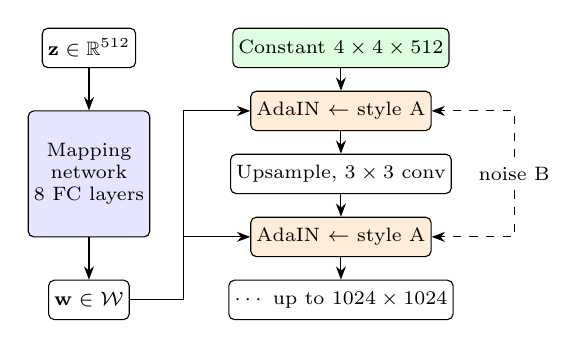
\begin{tikzpicture}[font=\scriptsize, >=Stealth,
  b/.style={draw, rounded corners=2pt, align=center, minimum height=0.5cm, inner sep=2pt}]
\node[b] (z) at (0,4.2) {$\mathbf{z}\in\mathbb{R}^{512}$};
\node[b, fill=blue!10, minimum height=1.6cm] (map) at (0,2.6) {Mapping\\network\\8 FC layers};
\node[b] (w) at (0,1.0) {$\mathbf{w}\in\mathcal{W}$};
\node[b, fill=green!12] (c) at (3.2,4.2) {Constant $4\times4\times512$};
\node[b, fill=orange!15] (a1) at (3.2,3.4) {AdaIN $\leftarrow$ style A};
\node[b] (cv) at (3.2,2.6) {Upsample, $3\times3$ conv};
\node[b, fill=orange!15] (a2) at (3.2,1.8) {AdaIN $\leftarrow$ style A};
\node[b] (dots) at (3.2,1.0) {$\cdots$ up to $1024\times1024$};
\node (n) at (5.4,2.6) {noise B};
\draw[->] (z) -- (map);
\draw[->] (map) -- (w);
\draw[->] (c) -- (a1);
\draw[->] (a1) -- (cv);
\draw[->] (cv) -- (a2);
\draw[->] (a2) -- (dots);
\draw[->] (w.east) -- (1.2,1.0) |- (a1.west);
\draw[->] (1.2,1.8) -- (a2.west);
\draw[->, dashed] (n) |- (a1.east);
\draw[->, dashed] (n) |- (a2.east);
\end{tikzpicture}
\caption{StyleGAN generator, simplified from~\cite{karras2019}. The mapping network turns $\mathbf{z}$ into $\mathbf{w}$, whose learned affine transforms (A) set the AdaIN styles of every layer. Per-pixel noise (B) adds random detail.}
\label{fig:style}
\end{figure}

\textbf{Mapping network.} Instead of feeding $\mathbf{z}$ directly into the generator, an 8-layer MLP maps it to an intermediate latent vector $\mathbf{w}$, with both spaces 512-dimensional~\cite{karras2019}. Because $\mathbf{w}$ does not have to follow a fixed prior, the space $\mathcal{W}$ can become less entangled, meaning that its directions correspond more directly to individual factors such as pose or hair color.

\textbf{Adaptive instance normalization.} The synthesis network starts from a learned $4\times4\times512$ constant rather than from $\mathbf{z}$. At each resolution, learned affine transforms turn $\mathbf{w}$ into a style $\mathbf{y}=(\mathbf{y}_s,\mathbf{y}_b)$ that modulates each feature map $\mathbf{x}_i$ through AdaIN~\cite[Eq.~1]{karras2019}:
\begin{equation}
\mathrm{AdaIN}(\mathbf{x}_i,\mathbf{y})=\mathbf{y}_{s,i}\,\frac{\mathbf{x}_i-\mu(\mathbf{x}_i)}{\sigma(\mathbf{x}_i)}+\mathbf{y}_{b,i}.
\end{equation}
Each feature map is first normalized to zero mean and unit variance and then rescaled and shifted by the style. Styles applied at low resolutions control coarse attributes such as pose and face shape, and styles at high resolutions control fine details such as color and texture.

\textbf{Noise, mixing, and truncation.} Single-channel Gaussian noise images are added after each convolution to produce random details such as hair placement and freckles without changing identity~\cite{karras2019}. During training, style mixing switches from one latent vector to another at a random layer, which prevents neighboring layers from relying on each other. At generation time, the truncation trick $\mathbf{w}'=\bar{\mathbf{w}}+\psi(\mathbf{w}-\bar{\mathbf{w}})$, with $\psi<1$, pulls $\mathbf{w}$ toward the average $\bar{\mathbf{w}}$, trading diversity for quality.

\textbf{Results.} StyleGAN reduced the FID from 8.04 for the Progressive GAN baseline to 4.40 on the FFHQ face dataset, and from 7.79 to 5.17 on CelebA-HQ~\cite{karras2019}. It also reduced the perceptual path length, a measure of how smoothly images change along the latent space, from 412.0 for a traditional generator to 234.0, a reduction of 43\%~\cite{karras2019}. The authors also introduced FFHQ, a dataset of 70,000 high-quality face images at $1024\times1024$.

\subsection{Comparison}
Table~\ref{tab:compare} summarizes the six models. The mathematical line of work (GAN to WGAN-GP) changed the objective to give stable, informative gradients. The architectural line (DCGAN to StyleGAN) changed the networks to improve image quality and control. The two lines are complementary: modern models combine improved losses with improved architectures.

\begin{table}[t]
\centering
\caption{Comparison of the analyzed GAN variants}
\label{tab:compare}
\setlength{\tabcolsep}{2.5pt}
\begin{tabular}{llp{2.3cm}p{2.1cm}}
\toprule
Model & Distance & Key idea & Reported result \\
\midrule
GAN~\cite{goodfellow2014} & JSD & adversarial game, MLPs & MNIST Parzen $225\pm2$ \\
cGAN~\cite{mirza2014} & JSD (conditional) & condition on label $\mathbf{y}$ & MNIST Parzen $132\pm1.8$ \\
DCGAN~\cite{radford2016} & JSD & strided convs, BN, LeakyReLU & 82.8\% CIFAR-10 (features) \\
WGAN~\cite{arjovsky2017} & Wasserstein-1 & critic, weight clipping & no mode collapse observed \\
WGAN-GP~\cite{gulrajani2017} & Wasserstein-1 & gradient penalty, $\lambda=10$ & IS $7.86$ CIFAR-10 \\
StyleGAN~\cite{karras2019} & --- & mapping net, AdaIN, noise & FID 4.40 FFHQ \\
\bottomrule
\end{tabular}
\end{table}

\section{Practical Applications}
\textbf{Image generation.} The most direct application is generating realistic images. StyleGAN produces faces at $1024\times1024$ that are difficult to distinguish from photographs, and its controllable styles allow editing attributes such as age or pose~\cite{karras2019}.

\textbf{Super-resolution.} SRGAN reconstructs high-resolution images from low-resolution inputs~\cite{ledig2017}. Models trained only with pixel-wise losses produce blurry results, because they average over many plausible details. Adding an adversarial loss pushes the output onto the manifold of natural images, so that it contains sharp, realistic textures.

\textbf{Image-to-image translation.} Pix2pix uses a conditional GAN in which the input image is the condition, for example a map or a sketch, and adds an $L_1$ loss to stay close to the target: $G^*=\arg\min_G\max_D\mathcal{L}_{\mathrm{cGAN}}(G,D)+\lambda\mathcal{L}_{L_1}(G)$~\cite{isola2017}. When paired training images do not exist, CycleGAN learns two mappings $G:X\to Y$ and $F:Y\to X$ with a cycle-consistency loss $\E\|F(G(x))-x\|_1+\E\|G(F(y))-y\|_1$, which requires that translating an image and translating it back recovers the original~\cite{zhu2017}. This enables tasks such as turning horses into zebras or photos into paintings.

\textbf{Data augmentation and medical imaging.} Medical datasets are often small, because labeling requires experts and data is protected by privacy rules. Frid-Adar et al.\ trained GANs to synthesize computed tomography (CT) images of liver lesions from a dataset of 182 lesions~\cite{fridadar2018}. Adding the synthetic images to the training set raised a lesion classifier's sensitivity from 78.6\% to 85.7\% and its specificity from 88.4\% to 92.4\%, compared with classic augmentation alone.

\textbf{Synthetic data.} More generally, GANs can create synthetic datasets that preserve the statistics of real data. These can balance rare classes, test systems on varied inputs, or share data when the original cannot be released. Synthetic data still needs careful checks, because a generator can memorize training samples or miss rare cases, and mode collapse in particular reduces diversity.

\section{Conclusion}
GANs turn generative modeling into a game between a generator and a discriminator. With an optimal discriminator, the game minimizes the Jensen--Shannon divergence and has a unique equilibrium where the generated distribution equals the data distribution. The derivations also explain GANs' practical weaknesses. The JSD is constant for non-overlapping distributions and the minimax loss saturates, which causes vanishing gradients. The game may oscillate instead of converging, and the generator can collapse onto a few modes. The papers analyzed here address these problems from two directions. DCGAN and StyleGAN improved the architectures, which led to stable convolutional training and controllable photorealistic images. WGAN and WGAN-GP improved the objective, replacing the JSD with the Wasserstein distance and enforcing the Lipschitz constraint with a gradient penalty. Together, these advances made GANs a practical tool for image generation, super-resolution, translation, and data augmentation, including in medical imaging.

\bibliographystyle{IEEEtran}
\bibliography{references}

\end{document}
